%\setcounter{section}{4}
%\setcounter{subsection}{4}
%\setcounter{subsubsection}{4}
%\setcounter{equation}{4}
%\pagenumbering{arabic} 
%\setcounter{page}{0}    %%%%%KKD used \setcounter{page}{0}  
%\oddsidemargin 0.9 cm 
%\evensidemargin -.4 cm
%\setlength{\textwidth}{152.4 mm}
 
\chapter{The Compact Muon Solenoid \label{The Compact Muon Solenoid}}

\section{CMS detector}
The Compact Muon Solenoid (CMS) ~\cite{cms-jinst} is one of the general purpose detectors at the Large Hadron Collider (LHC)~\cite{theLHC}, CERN near Geneva, Switzerland. The LHC is considered to be the most efficient and controlled instrument with which one can probe fundamental physics of high energy collisions. Its main job is to accelerate two energetic beams of charged particles (protons or lead ions) and to let them collide at few well defined points. The CMS detector sits at one point and records all the possible interesting events that results from these collisions. It is 21.6 m long, 15 m in diameter, and weighs about 14 kilotons. Approximately 3,800 people, representing 199 scientific institutes from 43 countries, form the CMS collaboration who built and now operate the gigantic detector. It comprises of subsystems, well designed to measure the energy and momentum of photons, electrons, muons, and other products of the collisions. It is located in an underground cavern at Cessy in France, just across the border from Geneva. Studies presented in this thesis are based on proton-proton collision data collected by the CMS experiment at $\sqrt(s)$ of 13 TeV. Two pictures of the detector are shown in Figs.~\ref{fig:CMSdetector1Thesis} and ~\ref{fig:CMSdetector2}. More details about the CMS detector can be found from the Ref.~\cite{physics-tdr-8.1, physics-tdr-8.2}.
\begin{figure}[h]
    \centering
    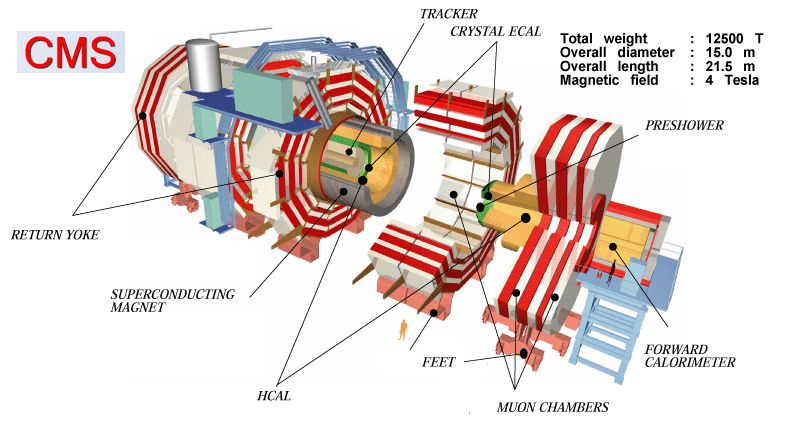
\includegraphics[width=16.0cm,height=8cm]{/home/bibhu/Desktop/PhDThesis/PhDThesis/chapter4/cms_detector.png}
    \caption{ \small An inside view of the CMS detector, showing various subdetectors that are placed around the beam pipe and form a series of cylindrical layers of the experiment. This image is taken from Ref.~\cite{cms-det}.}
    \label{fig:CMSdetector1Thesis}
\end{figure}


\begin{figure}[h]
    \centering  
    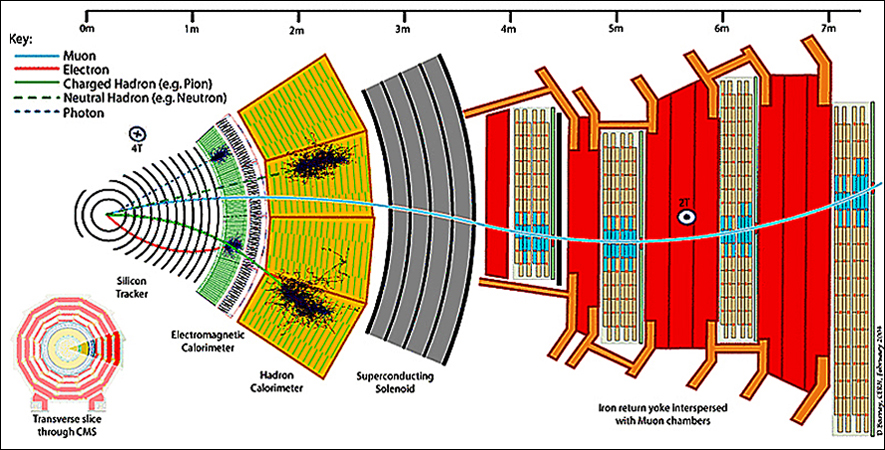
\includegraphics[width=15.0cm,height=6.8cm]{/home/bibhu/Desktop/PhDThesis/PhDThesis/chapter4/cms_slice.jpg}
    \caption{ \small Various detector components that contribute to event reconstruction are (from left to right) tracker, electromagnetic calorimeter,hadron calorimeter, superconducting solenoid and muon system. The paths of different particles  such as photons, muons, electrons, neutral and charged hadrons passing through the detector indicated by different solid or dashed color lines.}
    \label{fig:CMSdetector2}
\end{figure}
CMS has four major subcomponents, namely 

\begin{itemize}

\item Tracker,
\vspace{0.1cm} 
\item Electromagnetic calorimeter
\vspace{0.1cm} 
\item Hadron calorimeter, and 
\vspace{0.1cm} 
\item Muon system.


\end{itemize}

We shall now explain the individual components of the detector one by one. 


\subsection{Tracker}

The innermost part of the CMS detector is a silicon tracking system places at an approximate distance of 10 cm from the IP. It infers the momentum of charged particles by measuring their bending in presence of the magnetic field. It also plays an important role in identifying the number of primary vertices present in each event and helps reduce the pileup contamination in the event. The Figure.~\ref{fig:CMSdetector1Thesis} shows the position of tracker in the CMS detector. It is 5.8 m long and 2.5 m in diameter, centered around the interaction point (IP). It is designed to provide a robust, efficient and precise measurement of the  trajectories of charged particles. Tracker consists of  two main subcomponents namely pixel and microstrip detector. The tracker covers up to $|\eta| < $ 2.5.  The pixel detector helps to detect the secondary vertices and hence to identify jets initiated by a b-quark (b-jets). On the other hand, the microstrip detector is a key to the momentum measurement.



\begin{figure}[h]
    \centering  
    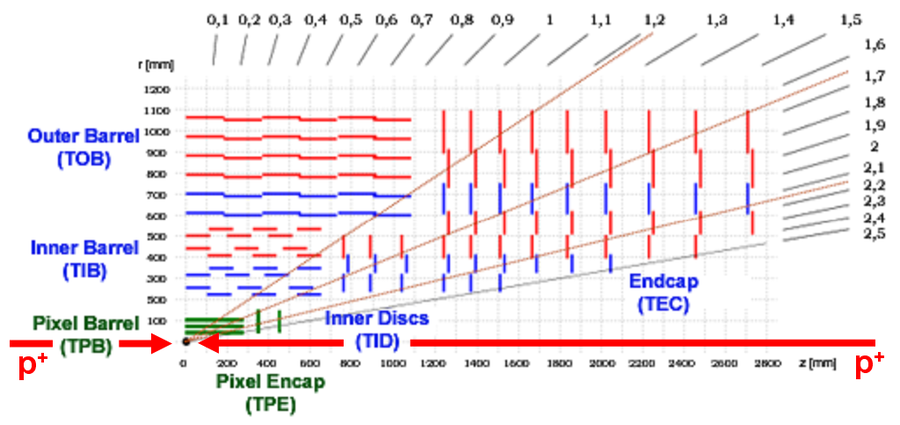
\includegraphics[width=15.0cm,height=6.0cm]{/home/bibhu/Desktop/PhDThesis/PhDThesis/chapter4/CMSQTracker.png}
    \caption{ \small A schematic diagram of the CMS Tracker. The plot shows one quadrant of the tracking detector along the $rz$ plane.}
    \label{fig:CMSQTracker1}
\end{figure}


The central part of the tracking detector is called barrel which has a cylindrical shape with the axis of symmetry coinciding with the LHC beamline and consists of three layers. In the forward and backward regions there are two endcaps each comprising two layers of pixels. The pixel detector consists of in total 66 million pixels. It is capable of detecting particles within the  pseudorapidity range $|\eta| \leq$ 2.4 with average spatial resolution of 10 $\mu m$ along the transverse $\rm r\phi$ plane and 20 $\mu m $ along the z direction.

As the distance from the IP increases the particle flux decreases and tracking job is done by a silicon microstrip detector that surrounds the pixel detector. It consists of 10 barrel layers (4 TIB-Tracker Inner Barrel and 6 TOB (Tracker Outer Barrel), 3 TID (Tracker Inner Disks)  and 9 TEC (Tracker Endcap) disks. A schematic diagram of the cross sectional slice of one quarter is shown in Fig.~\ref{fig:CMSQTracker1}. More details about tracker can be found in Ref.~\cite{physics-tdr-8.1}.  


\subsection{Electromagnetic Calorimeter}

Calorimeters (energy measuring devices) can be divided into two categories: homogeneous if the whole detector volume is active , and sampling, if the detector mostly comprises a passive absorber with only a fraction consisting of active volume. The CMS electromagnetic calorimeter (ECAL) is a homogeneous type that provides excellent energy and position measurements for photons and electrons. The active materials of the ECAL are lead tungstate ($PbWO_{4}$)  crystals providing around 25 radiation lengths($X_{0}$). A particle entering the ECAL results in an electromagnetic shower caused by the successive processes of bremsstrahlung and pair production. At the end, the energy of the particle is deposited in the calorimeter material via ionization and photoelectric effect. An electromagnetic shower is the process through which an energetic electromagnetic particle interacts with matter generating a cascade process composed of large number of secondary particles (photons, electrons and positrons). This occurs because electrons and positrons having energy greater than 1 GeV lose energy mostly via bremsstrahlung while photons via pair production. The secondary particles produced by the primary ones interact through the same process leading to the development of a particle shower inside the calorimeter. 


The CMS ECAL consists of 75848 $\it PbWO_{4}$ crystals. The radiation length of this crystal is 0.89 cm. The lateral spread of the shower is depends on the Moliere radius ($\rm R_{M}= 2.2 cm$) of the material. The light emission is fast enough to work with the highest LHC bunch crossing rate of 25 ns. 

The ECAL has two parts :  barrel (EB) extending up to $|\eta| < 1.479$ and ECAL endcap (EE) covering $|\eta|$ from 1.479 to 3.0.  For a better discrimination of photons against neutral pions, a preshower device(ES) is mounted in front of EE. In ES silicon millistrip sensors with a resolution of 2mm, placed behind two planes of lead, are able to distinguish single photons from $\pi^{0}$s decaying into photon pairs.

\begin{figure}[H]
    \centering  
    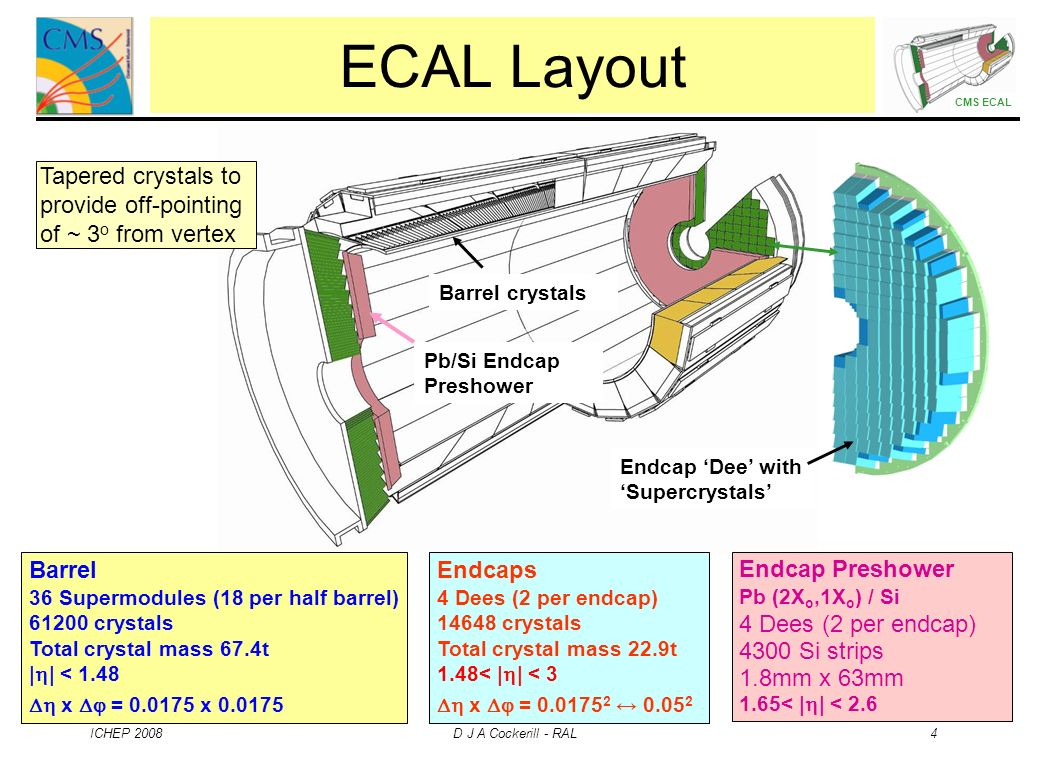
\includegraphics[width=16.0cm,height=8cm]{/home/bibhu/Desktop/PhDThesis/PhDThesis/chapter4/CMSecal.jpg}
    \caption{ \small A schematic diagram of the CMS ECAL  showing its different components.}
    \label{fig:CMSecal}
\end{figure}


{\Large ECAL Performance }

The energy resolution of the CMS ECAL is given by  the following expression 


\begin{equation} \label{ecalresolution}
\it \frac{\sigma_{E}}{E} = \frac{S}{\sqrt{E}} \oplus \frac{N}{E} \oplus C
\end{equation}
 
where E is the energy in GeV, $S$=2.8\% is the stochastic term , $N$= 124 MeV is the noise term, and $C$ = 0.3\% is the constant term. Various sources of contributions to these three terms as follows.

{\bf Stochastic term}
\vspace{-0.2in}
\begin{itemize}
\item event-to-event fluctuations in the lateral shower containment \vspace{-0.2in}
\item a photo statistics contribution of 2.1\% \vspace{-0.2in}
\item fluctuations in the energy deposited in the ES absorber with respect to what is measured in the preshower silicon detector. \vspace{-0.2in}
\end{itemize} 

{\bf Constant term}
\vspace{-0.2in}
\begin{itemize}

\item non-uniformity of longitudinal light collection \vspace{-0.2in}

\item intercalibration errors \vspace{-0.2in}

\item leakage of the energy from the back of the crystal \vspace{-0.2in}

\end{itemize} 


{\bf Noise term}
\vspace{-0.2in}

\begin{itemize}

\item electronics noise \vspace{-0.2in}

\item digitization noise \vspace{-0.2in}

\item pileup noise \vspace{-0.2in}
\end{itemize} 

The ECAL material budget and energy resolution vs. pseudorapidity is show in Fig.~\ref{fig:ResolutionECAL}.

\begin{figure}[H]
    \centering  
    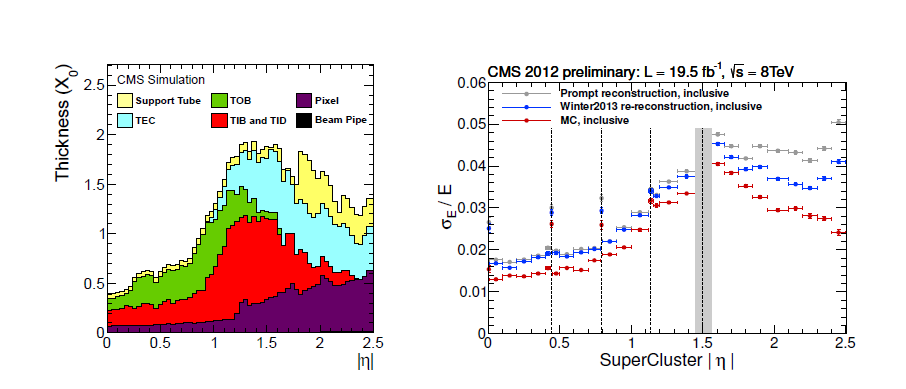
\includegraphics[width=16.0cm,height=8cm]{/home/bibhu/Desktop/PhDThesis/PhDThesis/chapter4/ResolutionECAL.png}
    \caption{ \small Amount of material (in units of radiation lengths) upstream of the ECAL (left). ECAL energy
resolution (right) as a function of pseudorapidity for electrons from $Z\rightarrow e^{+}e^{-}$ decays. The energy resolution
estimated on Monte Carlo events is shown in red, while in blue and gray the resolution for, respectively, promptly reconstructed
data and a later reconstruction of the same sample upon the usage of the best calibrations
available are shown.}
    \label{fig:ResolutionECAL}
\end{figure}



\subsection{Hadron Calorimeter}

The Hadron Calorimeter (HCAL) measures the energy of hadrons, particles made of quarks and gluons, for example protons, neutrons, pions and kaons. Additionally, it provides an indirect measurement for non-interacting, uncharged particles such as neutrinos. The HCAL consists of layers of dense material (brass or steel) interleaved with tiles of plastic scintillators, which are read out via wavelength-shifting   fibres by hybrid photodiodes. This combination was decided to allow the maximum amount of absorbing material inside of the magnet coil. The high pseudorapidity region ($3.0 < |\eta| < 5.0$)   is instrumented by the Hadronic Forward (HF) detector. It uses a slightly different technology of steel absorbers and quartz fibres for readout, designed to allow a better separation of particles in the congested forward region. The HF is also used to measure online, the relative luminosity system in CMS.

The HCAL is not only used to measure single hadrons but also jets with good precision. Jets are complex objects made of a mixture of particles such as hadrons, electrons, photons and muons, originating from the interaction of partons during hadron-hadron collisons. Achieving good precision for their energy scale and resolution is of crucial importance for many physics analyses and poses a big challenge for the HCAL  design. The CMS HCAL is a sampling calorimeter surrounding the Traker and ECAL. It reconstructs both charged and neutral hadrons produced during pp collisions. Brass has been chosen as the absorber material for the HCAL as it is non-magnetic and has a relatively short interaction length of $\lambda_{I} = $ 16 cm. The large fraction of passive material is cost efficient. The HCAL has four main subcomponents as shown in Fig.~\ref{fig:HCALLV}

\begin{figure}[h]
    \centering  
    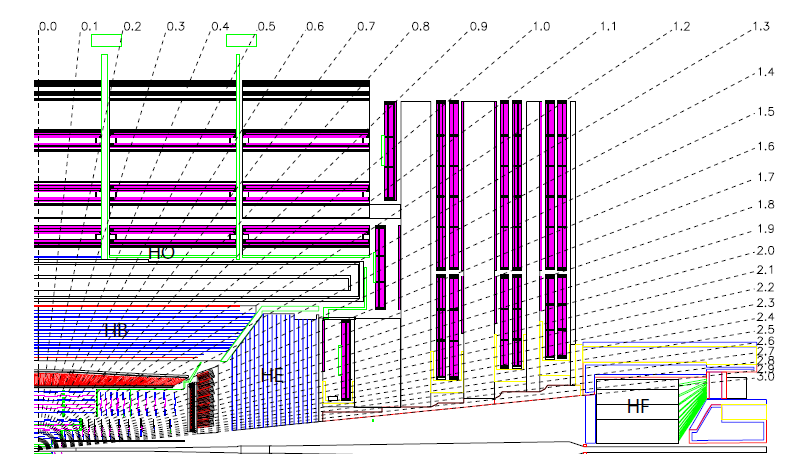
\includegraphics[width=15.0cm,height=8cm]{/home/bibhu/Desktop/PhDThesis/PhDThesis/chapter4/HCALLV.png}
    \caption{ \small A schematic diagram of the CMS HCAL showing its individual components.}
    \label{fig:HCALLV}
\end{figure}

The subcomponents are Hadron Barrel (HB), Hadron Outer (HO), Hadron Endcap (HE) and Hadron Forward (HF). HB is the inner part of the HCAL barrel with $1.305 < |\eta|<1.392$. HO helps to measure the energy of hadron showers penetrating the magnetic coil. It extends up to $|\eta| $=1.26. HE has 14 additional calorimeter towers covering the pseudorapidity region $1.3 <|\eta|<3.0$. To cover higher $\eta$ range $2.8<|\eta|<5.2$, HF is located at $ z= \pm 11.2 \rm m$ from the IP close to the beam pipe. Jets with very high $|\eta|$ values as well as the hadronization products of beam remnants are detected with this system.


{\bf HCAL Performance}

The hadron energy resolution for the barrel HCAL and ECAL combination can be given as 

\begin{equation} \label{hcalresolution}
\it \frac{\sigma_{E}}{E} = \frac{a}{\sqrt{E}}  \oplus b 
\end{equation}

where $a$ is the stochastic term and $b$ is the constant term, measured in the test beam as $0.847\pm 0.016$ $\sqrt{\rm GeV}$ and $0.074 \pm 0.008$, respectively.


\subsection{Muon System}

As the name `Compact Muon Solenoid' suggests, detecting muons is one of the most important tasks for CMS. Muons are minimum interacting particles that can pass through several metres of iron   without much energy loss  and are not stopped by two calorimeters of CMS. Therefore, gas-based chambers to detect muons are placed at the very edge of the experiment where they are the only particles likely to register a signal. 

To identify muons and measure their momenta, CMS uses three types of detector: drift tubes (DTs), cathode strip chambers (CSCs) and resistive plate chambers (RPCs). The DTs are used for precise trajectory measurements in the barrel region, while the CSCs are employed in the endcaps. The RPCs provide a fast (trigger) signal when a muon passes through the muon detector, and are installed in both the barrel and the endcaps.

{\bf Drift Tubes}

The muon barrel (MB) consists of four layers of DT chambers. Each chamber is 4 cm wide tube that contains a stretched wire within a gas volume. When a muon or any other charged particle passes through the volume, it knocks out electrons off the gas atoms. These electrons follow the electric field ending up at the positively-charged wire. By keeping track of the wire electrons hit as well as by calculating the muons' original distance away from the wire, the DTs give two coordinates for the muons' position.

{\bf Cathode Strip Chambers}

The muon endcap consists of 468 CSCs in two endcaps. The CSCs are used in the endcap disks where the magnetic field is irregular and the particle rates are very high. They consist of arrays of positively-charged anode wires crossed with negatively-charged copper cathode strips within a gas volume. When muons pass through, they knock electrons off the gas atoms, which flock to the anode wires creating an avalanche of electrons. Positive ions move away from the anode wire and towards the copper cathode, inducing a charge pulse in the strips, at right angles to the wire direction. Because the strips and the wires are perpendicular, we get two position coordinates for each passing particle.

In addition to providing precise space and time information, the closely spaced wires make the CSCs fast detectors suitable for triggering. Each CSC module contains six layers enabling it to accurately identify muons and match their tracks to those in the tracker. 


{\bf Resistive Plate Chambers}

RPCs are fast gaseous detectors that provide a muon trigger system parallel with those of the DTs and CSCs. They consist of two parallel plates, a positively-charged anode and a negatively-charged cathode, both made of a very high resistivity plastic material and separated by a gas volume.

When a muon passes through the RPC, electrons are knocked out of gas atoms. These electrons in turn hit other atoms causing an avalanche of electrons. The electrodes are transparent to the signal (due to electrons), which are instead picked up by external metallic strips after a small but precise time delay. The pattern of hit strips gives a quick measure of the muon momentum, which is then used by the trigger to make immediate decisions about whether the data are worth retaining. RPCs combine a good spatial resolution with a time resolution of just one nanosecond. Fig.~\ref{fig:MuonSystem} shows the schematic diagram of CMS muon system with position of CSCs, DTs and RPCs.


\begin{figure}[H]
    \centering
    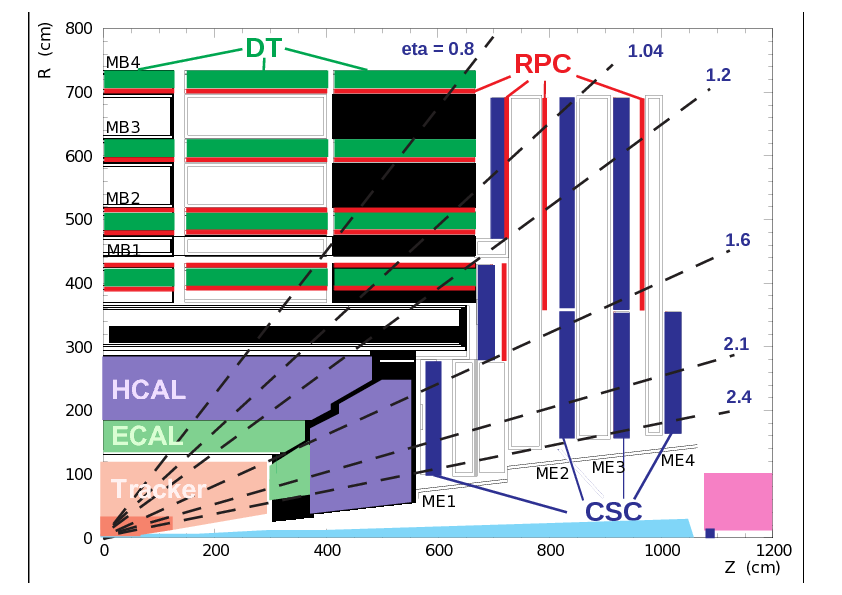
\includegraphics[width=15.0cm,height=10cm]{/home/bibhu/Desktop/PhDThesis/PhDThesis/chapter4/MuonSystemCMS.png}
    \caption{ \small CMS muon system and position of muon subdetectors. The image is taken from Ref.~\cite{MuonSysImage}.}
    \label{fig:MuonSystem}
\end{figure}

{\bf Muon System Performance}

The muon momentum is measured in the inner silicon tracker as well as in the muon system. When only used the muon system, a momentum resolution of 10\% (20\%) is achieved for 40 GeV muons in the barrel (endcaps). However, the resolution of a global muon that combines information from the tracker with the muon system, is about 1\% (2\%) for muons with $\rm p_{T} <$ 100 GeV in the barrel (endcaps). For high $\rm p_{T}$ muons (above 100 GeV), the resolution degrades to about 8\% for the barrel and 10 \% for the endcaps.





\section{Object Reconstruction}

In this section, we discuss generic methods that are used to reconstruct electron, muon, jets and MET in CMS. These methods remain the same for all  objects used throughout the analysis works presented here. Basically the these objects are reconstructed by studying the distributions of several variables that provide some information about the former. The exact criteria might change from analysis to analysis but the reconstruction methods remain unchanged.

\subsection{ Primary Vertex Reconstruction}

The goal of primary vertex reconstruction is to determine the hardest vertex i.e. the precise position of pp interaction point. This task is accomplished with the so called Deterministic Annealing ~\cite{PValgo} clustering of tracks. From a set of reconstructed vertices, the one with maximal $\sum p_{T}^{2}$ is chosen as the primary vertex or the collision point.




\subsection{Electron Reconstruction}

Electrons are identified by combining tracks in the silicon tracker with energy deposits in the ECAL. Track trajectories are reconstructed using a dedicated modeling of the energy-loss due to bremsstrahlung radiation within the tracker material, and are fitted with a gaussian sum filter (GSF)~\cite{GSF}. The electron track reconstruction is performed by collecting the hits and accessing all the track parameters of the tracks with a large spectrum of emitted bremsstrahlung photons. 

Electrons are identified using  the following track and cluster shape variables.
\begin{itemize}

\item The difference between the cluster position and the track extrapolation from the innermost measurement in the $\eta$ direction ($\Delta \eta_{in}$). \vspace{-0.2in}

\item The difference between the cluster position and the track extrapolation from the innermost measurement in the  $\phi$ direction ($\Delta \phi_{in}$). \vspace{-0.2in}

\item The cluster $\eta$ width ($\sigma_{i\eta i\eta}$), which is defined from the covariance matrix with logarithmic weights \vspace{-0.2in}

\item  The ratio of energy leaked into HCAL over the energy in the ECAL ($\it H/E$).\vspace{-0.2in}

\item The impact parameter in the transverse ($r\phi$) plane with respect to the primary vertex \vspace{-0.2in}

\item The impact parameter along the $\it z$-axis with respect to the primary vertex. 

\end{itemize}




\subsection{Muon Reconstruction}
Muon reconstruction is performed using the all-silicon inner tracker at the centre of the detector, and with up to four stations of gas-ionization muon detectors installed outside the solenoid and sandwiched between the layers of the steel return yoke ~\cite{MuonReco}. The muon system covers the pseudorapidity region $\eta < $ 2.4 and performs three main tasks: triggering on muons, identifying them, and improving their momentum measurement and charge determination.


\subsection{Jet Reconstruction}

All three analyses presented in this thesis use jets. In fact, jets constitute an important part of object reconstruction in CMS. First particles 
 (electrons, muons, photons, charged and neutral hadrons) are reconstructed using the Particle Flow (PF) method.~\cite{PFmethod}. These PF candidates are then fed to the anti-$k_{t}$ ~\cite{antiKT} jet reclustering algorithm to form jets. The cone radius for jet reconstruction in the SUSY and leptoquark analysis is taken to be 0.4. In the pileup mitigation study, however, the same is changed to 0.8.  To further improve their quality, a following set of criteria are imposed on our studies.

\begin{itemize}
\item Number of constituent particles in the jet should be greater than 1, \vspace{-0.2in}
\item Charged electromagnetic energy fraction in the jet should be less than 0.99, \vspace{-0.2in}

\item Neutral hadronic energy fraction in the jet should be less than 0.99, \vspace{-0.2in}

\item  Neutral electromagnetic energy fraction in the jet should be less than 0.99, \vspace{-0.2in}

\item Charged energy fraction in the jet should be greater than 0.0 within the $|\eta| < $ 2.4, and \vspace{-0.2in}

\item Charged multiplicity in the jet should be non-zero within $|\eta| < $2.4.\vspace{-0.2in}

\end{itemize}


\subsection{Missing Transverse Energy}

If a neutrino is present in the final state, it goes undetected in the detector. As a result, when we add up the momentum of all visible particles in the transverse plane, there is an overall imbalance. The amount needed to balance the transverse momentum to zero decides the MET ($E_{T}$) of the event. So $E_{T}$ is computed as the negative vector sum of the transverse momenta of all PF candidates. The raw $E_{T}$ is corrected for to remove the bias due to non-linearity in the calorimetric response for neutral and charged hadrons, caused by pileup, large bending of low $p_{T}$ tracks due to the strong magnetic fields in the CMS. 









